\documentclass[]{article}
\usepackage[italian]{babel}
\usepackage[T1]{fontenc}
\usepackage[utf8]{inputenc}
\usepackage{hyperref}
\usepackage{graphicx}
\usepackage{float}
\usepackage{fancyhdr}
\usepackage{listings}
\usepackage{color}


%opening
\title{Architettura di MyDFS}
\author{Sedoni Enrico}


\begin{document}

\maketitle

\begin{abstract}

In questo articolo si descrive più a fondo il meccanismo introdotto per garantire un sistema tollerante ai guasti. In particolare vengono trattati i meccanismi per garantire consistenza e affidabilità nel sistema.

\end{abstract}


\tableofcontents
\newpage

\section{Architettura generale di MyDFS}

Si parte innanzitutto a spiegare l'architettura generale del sistema, per poi approfondire mano a mano nello specifico le varie componenti del sistema e come interagiscono tra di loro.

\setlength\parindent{0pt}
L'intero sistema è sviluppato secondo il principio architetturale \textbf{Master-Slave}.

\vspace{1.5cm}
\setlength\parindent{0pt}
Di seguito viene mostrata l'architettura generale:

\begin{figure}[h]
	\centering
	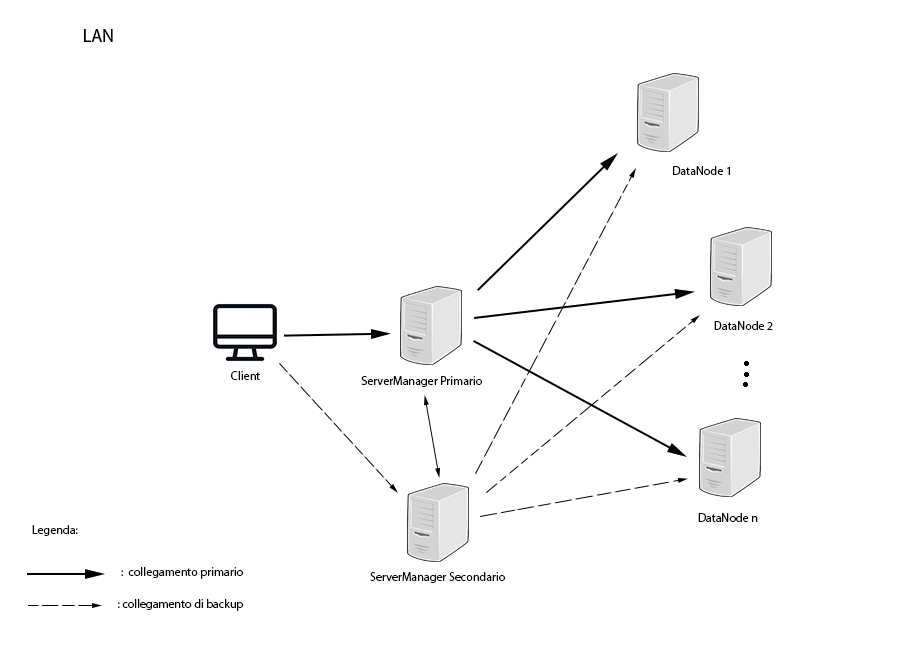
\includegraphics[width=16cm]{../Img/ArchitetturaMyDFS}
	\caption[]{Architettura di MyDFS}
	\label{fig:ArchitetturaMyDFS}
	
\end{figure}


\subsection{Componenti del sistema}

Il sistema presenta tre tipologie di macchine:

\begin{itemize}
		\item \textit{\textbf{DataNode}}: è il nodo che si occupa della gestione dei file a livello locale. Si occupa quindi di creare file, eliminarli, spostarli e copiarli all'interno del file system locale gestito. È coordinato dal ServerManager. All'interno del codice è identificato dalla classe con il nome "ServerClass". Svolge la funzione di Slave.
		\item \textit{\textbf{ServerManager}}: è il nodo che coordina i vari Data Nodes appartenenti al sistema e che comunica direttamente e gestisce i vari client. Il suo compito è quello di gestire l'allocazione dei dati tra i vari Data Nodes e avere quindi un carico bilanciato tra tutte le componenti. Svolge la funzione di Master.
		\item \textit{\textbf{Client}}: è il processo client del sistema
		
\end{itemize}

Il serverManager è in grado di gestire un numero corposo di client allo stesso tempo e un numero di slave illimitato. Più slave saranno presenti nel cluster, più sarà lo spazio a disposizione disponibile. La grande scalabilità orrizzontale del sistema è quindi un vantaggio di questa particolare tipologia di architettura.

\subsubsection{Gestione dello stato}

Per non andare a complicare ulteriormente la logica del ServerManager e non andarlo a sovraccaricare di lavoro, si è deciso di optare per una soluzione \textbf{stateless}.
\vspace{0.2cm}

 Il ServerManager non mantiene quindi lo stato del client, questo è
 mantenuto direttamente all'interno del client stesso. In particolare viene mantenuto il percorso attuale del client all'interno del filesystem distribuito. Questa soluzione permette quindi di avere una gestione dei client multipli semplificata ed efficiente. 

\subsection{Layer di comunicazione}

Il sistema è diviso quindi in due layer di comunicazione differenti:

\begin{itemize}
	\item \textit{\textbf{Client - ServerManagers}}: è il layer di comunicazione più esterno, in particolare il client effettua le richieste ed il ServerManager risponde. Per esempio se il client dà il comando "ls" il ServerManager interroga tutti i DataNodes, costruisce la risposta e la restituisce al Client.
		
	\item \textit{\textbf{ServerManagers - DataNodes}}: è il layer di comunicazione più interno, il ServerManager svolge il ruolo di client e i DataNodes svolgono i ruoli di Server. Il serverManager può interrogare i DataNodes, ma anche decidere come allocare i dati all'interno di questi e come spostarli all'interno di essi, in modo da mantenere una gestione bilanciata del carico.
	
\end{itemize}

\vspace{0.5cm}
Il ServerManager implementa quindi anche funzionalità di \textbf{load balancing}.
Un compito fondamentale del ServerManger è quello di mantenere consistente la stessa struttura di directory tra i vari Data Nodes.

\subsection{ServerManager Secondario}

Il sistema nel suo funzionamento più semplice è resistente a fallimenti solo nei Data Nodes, il serverManager è un single point of failure (SPOF). Per questo è stato introdotto un meccanismo per rendere più resistente questo punto debole. In particolare è possibile designare anche un server manager secondario, che viene attivato solo se il serverManager primario crasha. Il ServerManager secondario assume quindi, temporaneamente, il ruolo di ServerManager primario, fino a quando quello originale non ripristina il suo funzionamento.

\newpage
\section{Fault tollerance e consistenza}

In questo capitolo viene spiegato nel dettaglio il meccanismo complesso introdotto nel sistema per supportare la tolleranza ai guasti, viene spiegato anche come si mantiene la consistenza tra i DataNodes e i ServerManagers.

\subsection{Classe Tree}

La classe Tree è il primo componente fondamentale da introdurre. Sta alla base di tutto quanto. Ogni nodo del sistema mantiene salvato in un file il FileSystemTree di sè stesso (si trova in /home/mydfsUser/.config/MyDFS). Sucessivamente ne verrà spiegata la motivazione.

Il fileSystemTree è sostanzialmente un albero nel quale ogni nodo rappresenta una directory.
\vspace{0.2cm}

Con la seguente immagine si chiarisce ogni dubbio:

\begin{figure}[h]
	\centering
	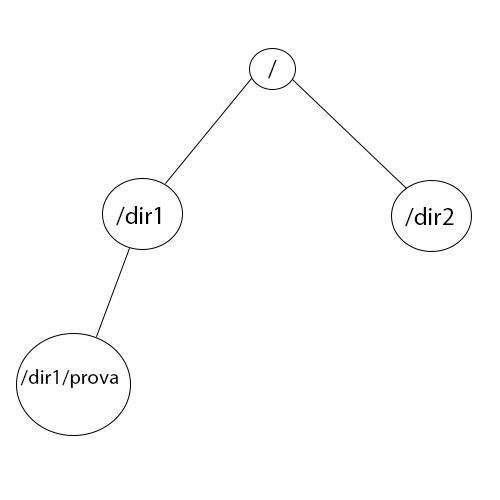
\includegraphics[width=6cm]{../Img/fileSystemTree.png}
	\caption[]{Esempio di fileSystemTree}
	\label{fig:fileSystemTree}
	
\end{figure}

Ogni nodo possiede due attributi:

\begin{itemize}
	\item \textit{Path}: percorso completo della directory all'interno del fileSystem
	\item \textit{Name}: nome della directory all'interno del fileSystem
\end{itemize}


La classe Tree implementa i metodi fondamentali per la gestione dei nodi all'interno dell'albero: cancellazione, inserimento, movimento, stampa, ricerca, etc..

\vspace{0.5cm}

la classe è serializzabile, in questo modo è possibile salvarla facilmente in un file e poi caricarla in memoria sucessivamente quando ce n'è il bisogno.

\subsection{Controllo della consistenza}

Il controllo della consistenza, anche chiamato "consistency check" all'interno del software, viene eseguito ogni volta che un nodo ServerManager/Data Nodes viene avviato ed entra a far parte della rete. Il ServerManager primario in particolare mantiene salvato il \textbf{fileSystemTree}, che ad ogni operazione che svolge il client può venire modificato. 

\vspace{0.2cm}
Anche i Data Nodes mantengono salvato il proprio fileSystemTree (file differente chiamato "fileSystemTreeSlave"), questo perchè se lo slave crasha e il client continua a svolgere operazioni, potrebbe rimanere indietro. Ad ogni avvio di uno slave, il suo fileSystemTree viene quindi confrontato con quello del ServerManager, se è differente questo viene aggiornato con quello del ServerManager.


\vspace{0.3cm}

Il fileSystemTree del ServerManger è quindi il principale ed è sempre il più aggiornato. Una operazione che lo va a modificare viene poi propagata anche al fileSystemTree dello slave successivamente.

\subsection{Fault Tollerance}

Per avere tolleranza ai guasti sono stati introdotti meccanismi complessi che fanno uso di più thread contemporaneamente per aggiornare e controllore lo stato dei Data Nodes e dei ServerMangers. In particolare sono state introdotte delle classi che implementano il funzionamento di questi thread:

\begin{itemize}
	\item  \textit{AsyncServerChecker}
	\item  \textit{ReconnecterThread}
	\item  \textit{ServerConnectedChecker}
	\item  \textit{SecondaryServerUpdater}
\end{itemize}

Di seguito ne viene spiegato il loro funzionamento e scopo nel dettaglio.

\subsubsection{AsyncServerChecker}

È il thread che si occupa di controllare ogni 100ms lo stato dei nodi slave (Data Nodes) all'interno della rete e connessi con il ServerManager. Questo thread viene quindi lanciato dal ServerManager primario, il quale è l'unico che possiede le informazioni sui nodi slave appartenenti alla rete in quel momento.

\vspace{0.3cm}
Di seguito viene mostrato il suo funzionamento attraverso un'immagine esemplificativa:

\begin{figure}[h]
	\centering
	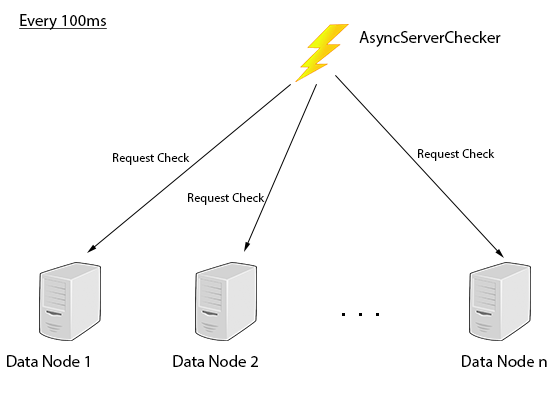
\includegraphics[width=8cm]{../Img/AsyncServerChecker1.png}
	\caption[]{AsyncServerChecker1 funzionamento}
	\label{fig:AsyncServerChecker1}
	
\end{figure}


\vspace{3cm}

Ma cosa succede se un Data Node crasha?

\begin{figure}[h]
	\centering
	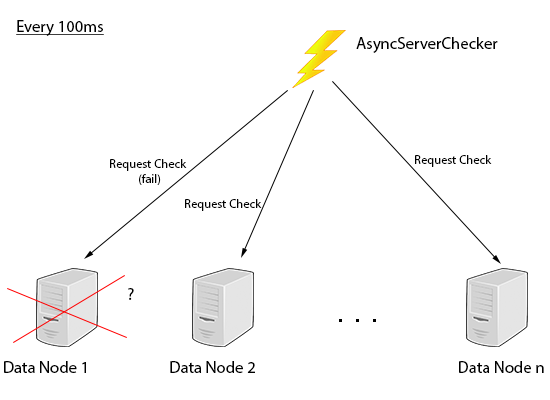
\includegraphics[width=8cm]{../Img/AsyncServerChecker_crash.png}
	\caption[]{AsyncServerChecker1 funzionamento}
	\label{fig:AsyncServerChecker_crash}
	
\end{figure}

\vspace{0.5cm}

Il ServerManager lancia un thread secondario chiamato \textbf{ReconnecterThread} e rimuove dalla lista degli SlaveNodes attualmente disponibili il nodo crashato.


\subsubsection{ReconnecterThread}

È un thread molto semplice, con il funzionamento di provare a ricontattare ogni secondo il nodo slave crashato (fig. \ref{fig:ReconnecterThread}), se questo torna online e quindi raggiungibile nuovamente, vengono svolte le seguenti operazioni:

\begin{itemize}
	\item aggiungo nuovamente il Data Node alla lista dei nodi slave raggiungibili del ServerManager
	\item controllo della consistenza del fileSystemTreeSlave con il fileSystemTree del ServerManager
	\item si effettuano eventuali correzioni del fileSystemTreeSlave se questo non è consistente
\end{itemize}


\begin{figure}
	\centering
	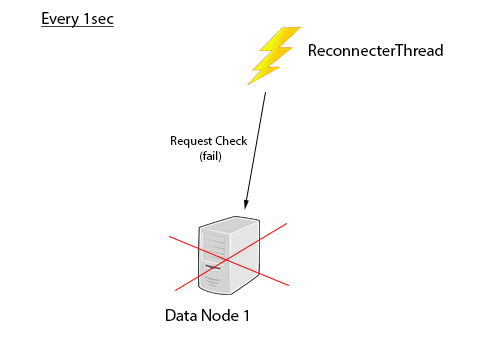
\includegraphics[width=8cm]{../Img/ReconnecterThread.png}
	\caption[]{ReconnecterThread funzionamento}
	\label{fig:ReconnecterThread}
	
\end{figure}



\subsection{ServerConnectedChecker}

Com'è stato già spiegato nel capitolo precedente, il sistema ha la possibilità di utilizzare quello che è un serverManager secondario di backup, nel caso il ServerManager primario crashi, in questo modo il SPOF non persiste più e si ottiene un sistema complessivamente più affidabile.

\vspace{0.5cm}

L'introduzione di questo server secondario tuttavia complica e non di poco la logica complessiva del software.

Questo thread viene lanciato dal processo client e si occupa di andare a controllare lo stato del ServerManager attraverso una richiesta "dummy" (in questo caso si prova a chiamare il metodo getName()), se la richiesta genera una eccezione vuol dire che si è verificato un problema nel serverManager e non è più raggiungibile. Il client viene quindi spostato nel serverManager secondario di backup, se specificato.

In particolare vengono svolti i seguenti step:

\begin{itemize}
	\item ogni secondo si manda una richiesta "dummy" per il check della salute del serverManager (fig. \ref{fig:ServerConnectedChecker1})
	\item se provoca una eccezione, il serverManager primario è fallito (fig. \ref{fig:ServerConnectedChecker2})
	\item si prova a verificare se il serverManager secondario è online e in funzione
	\item in caso di successo il serverManager secondario diventa il nuovo primario e il primario diventa secondario (swap) , il controllo del client passa quindi al nuovo serverManager primario (fig. \ref{fig:ServerConnectedChecker3})
	\item il primario crashato viene comunque controllato ogni secondo con una richiesta dummy
	\item se il primario torna online, la richiesta ha successo e il client passa di nuovo su questo server, primario e secondario vengono swappati nuovamente
\end{itemize}

\begin{figure}
	\centering
	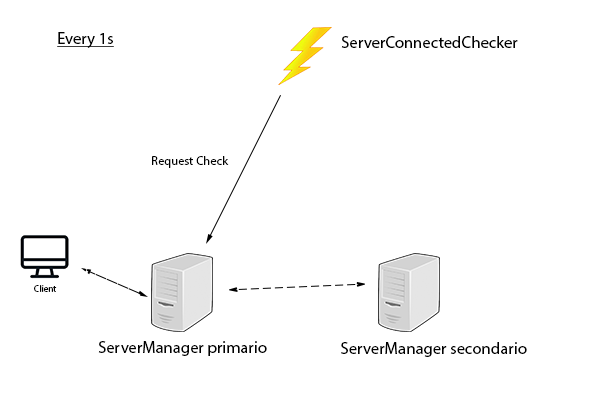
\includegraphics[width=8cm]{../Img/ServerConnectedChecker1.png}
	\caption[]{ServerConnectedChecker funzionamento}
	\label{fig:ServerConnectedChecker1}
	
\end{figure}
\begin{figure}
	\centering
	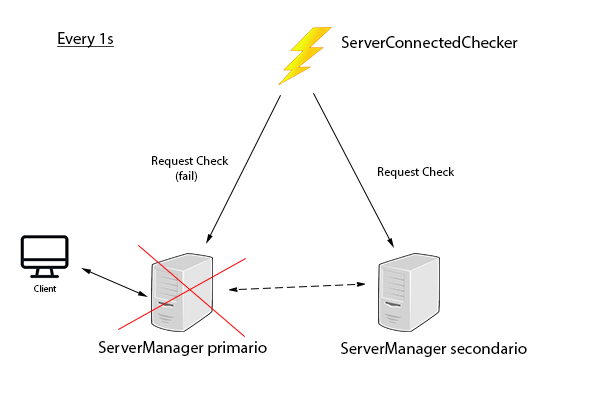
\includegraphics[width=8cm]{../Img/ServerConnectedChecker2.png}
	\caption[]{ServerConnectedChecker crash}
	\label{fig:ServerConnectedChecker2}
	
\end{figure}
\begin{figure}
	\centering
	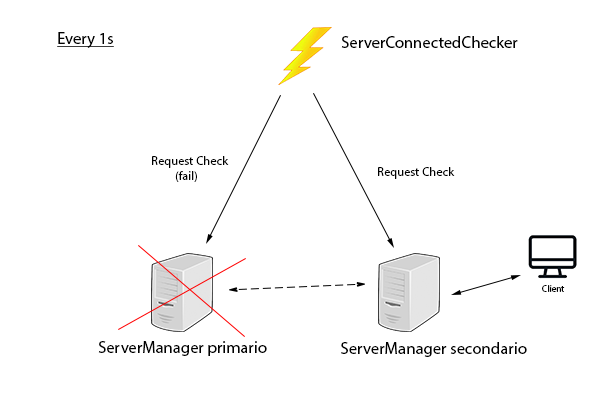
\includegraphics[width=8cm]{../Img/ServerConnectedChecker3.png}
	\caption[]{ServerConnectedChecker funzionamento}
	\label{fig:ServerConnectedChecker3}
	
\end{figure}


Ma come si gestisce la consistenza tra i fileSystemTree dei due serverManager? Il client potrebbe modificare il fileSystemTree con delle operazioni e il serverManager primario quando torna online deve esserle in grado di vedere. È inoltre necessario tenere aggiornato costantemente il fileSystemTree del server secondario, in modo che sia sempre pronto ad entrare in azione. Qui entra il gioco il quarto ed ultimo thread \textbf{SecondaryServerUpdater}

\subsection{SecondaryServerUpdater}

È un thread che entra in gioco solo nella modalità di funzionamento a due ServerManager. In particolare viene lanciato dal ServerManager primario e ogni 550ms si occupa di fare l'update del FileSystemTree del serverManager secondario (fig. \ref{fig:SecondaryServerUpdater}).


\begin{figure}[h]
	\centering
	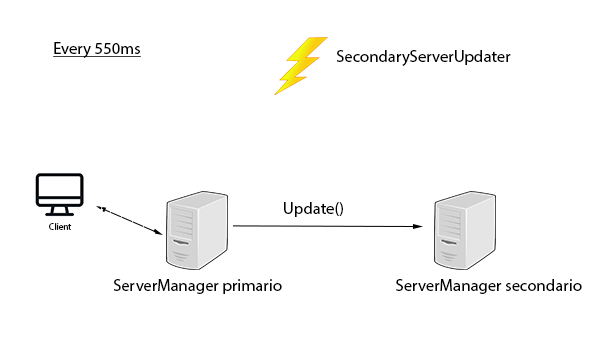
\includegraphics[width=8cm]{../Img/SecondaryServerUpdater.png}
	\caption[]{SecondaryServerUpdater funzionamento}
	\label{fig:SecondaryServerUpdater}
	
\end{figure}

Se il serverManager primario crasha, il controllo del client viene passato al serverManager secondario dal thread "ServerConnectedChecker" (fig. \ref{fig:SecondaryServerUpdater2}).



\begin{figure}
	\centering
	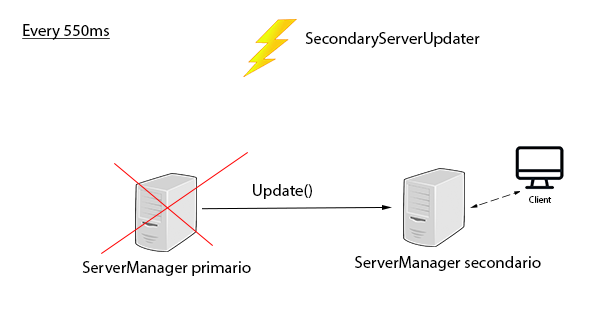
\includegraphics[width=8cm]{../Img/SecondaryServerUpdater2.png}
	\caption[]{SecondaryServerUpdater funzionamento}
	\label{fig:SecondaryServerUpdater2}
	
\end{figure}

\vspace{0.5cm}
NB: il serverManager secondario deve ricaricare in memoria il fileSystemTree aggiornato (con la funzione apposita "reloadFileSystemTree") prima di iniziare a lavorare

\vspace{1cm}


Se il serverManager primario torna online
\begin{itemize}
	
	\item il primario recupera il fileSystemTree dal secondario (fig. \ref{fig:SecondaryServerUpdater3})
	
	\item contronto il fileSystemTree del primario con il secondario, se sono diversi vuol dire che è stato modificato ed devo aggiornare il fileSystemTree del primario
	
	\item viene controllata la consistenza dei Data Nodes (ad ogni avvio di un serverManager)
	
	\item riprendo a comunicare con il client, il quale è stato spostato dal ServerManager secondario al primario nuovamente dal thread "ServerConnectedChecker"
	
\end{itemize}


\begin{figure}[h]
	\centering
	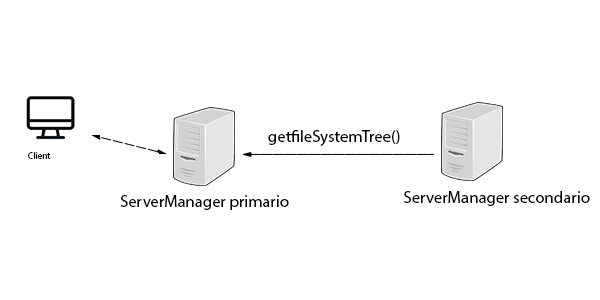
\includegraphics[width=8.6cm]{../Img/SecondaryServerUpdater3.png}
	\caption[]{SecondaryServerUpdater funzionamento}
	\label{fig:SecondaryServerUpdater3}
	
\end{figure}



\end{document}
